\documentclass[a4paper, 12pt]{article}%тип документа

%%%Библиотеки
	%\usepackage[warn]{mathtext}	
	\usepackage[T2A]{fontenc} % кодировка
	\usepackage[utf8]{inputenc} % кодировка исходного текста
	\usepackage[english,russian]{babel} % локализация и переносы
	\usepackage{caption}
	\usepackage{listings}
	\usepackage{amsmath,amsfonts,amssymb,amsthm,mathtools}
	\usepackage{wasysym}
	\usepackage{graphicx}%Вставка картинок правильная
	\usepackage{float}%"Плавающие" картинки
	\usepackage{wrapfig}%Обтекание фигур (таблиц, картинок и прочего)
	\usepackage{fancyhdr} %загрузим пакет
	\usepackage{lscape}
	\usepackage{xcolor}
	\usepackage[normalem]{ulem}
	\usepackage{hyperref}

%%%Конец библиотек




%%%Настройка ссылок
	\hypersetup
	{
		colorlinks=true,
		linkcolor=blue,
		filecolor=magenta,
		urlcolor=blue
	}
%%%Конец настройки ссылок


%%%Настройка колонтитулы
	\pagestyle{fancy}
	\fancyhead{}
	\fancyhead[L]{Лабораторная работа}
	\fancyhead[R]{Талашкевич Даниил, группа Б01-009}
	\fancyfoot[C]{\thepage}
%%%конец настройки колонтитулы



							\begin{document}
						%%%%Начало документа%%%%


%%%Начало титульника
\begin{titlepage}

	\newpage
	\begin{center}
		\normalsize Московский физико-технический институт \\(госудраственный 			университет)
	\end{center}

	\vspace{6em}

	\begin{center}
		\Large Лабораторная работа по электричеству\\
	\end{center}

	\vspace{1em}

	\begin{center}
		\large \textbf{Спектры электрических сигналов (компьютер) [3.6.1]}
	\end{center}

	\vspace{2em}

	\begin{center}
		\large Талашкевич Даниил Александрович\\
		Группа Б01-009
	\end{center}

	\vspace{\fill}

	\begin{center}
	Долгопрудный \\2021
	\end{center}
	
\end{titlepage}
%%%Конец Титульника



%%%Настройка оглавления и нумерации страниц
	\thispagestyle{empty}
	\newpage
	\tableofcontents
	\newpage
	\setcounter{page}{1}
%%%Настройка оглавления и нумерации страниц


					%%%%%%Начало работы с текстом%%%%%%

\section{Аннотация}

$\textbf{Цель работы}$: изучить спектральный состав периодических электрических сигналов.

$\textbf{В работе используются}$: анализатор спектра (ПК), генератор прямоугольных импульсов и сигналов специальной формы, осциллограф.

В работе изучается спектральный состав периодических электрических сигналов различной формы: последовательности прямоугольных импульсов, последовательности цугов и амплитудно модулированных гармонических колебаний. Спектры этих сигналов наблюдаются с помощью промышленного анализатора спектра и сравниваются с рассчитанными теоретически. 

\section{Теоретические сведения}

Сколь угодно сложныи электрическии сигнал $\mathrm{V}$ (t) может быть разложен на более простые сигналы. В радиотехнике широко используется разложение сигнала V (t) на совокупность гармонических сигналов различных частот $\omega .$ Функция $\mathrm{F}(\omega)$, описывающая зависимость амплитуд отдельных гармоник от частоты, называется амплитуднои спектральнои характеристикои сигнала $\mathrm{V}(\mathrm{t})$. Представление сложного периодического сигнала в виде суммы дискретных гармонических сигналов в математике называется разложением в ряд Фурье.

Зная спектральныи состав $\mathrm{F}(\omega)$ периодическои последовательности некоторого импульса V (t), мы можем осуществить обратное преобразование Фурье: сложив отдельные гармоники со своими амплитудами и фазами, получить необходимую последовательность импульсов. Степень совпадения полученного сигнала с V (t) определяется количеством синтезированных гармоник: чем их больше, тем лучше совпадение.
Рассмотрим конкретные примеры периодических функции, которые будут предметом исследования в нашеи работе.

Рассмотрим конкретные примеры периодических функций, которые будут предметом исследования в нашей работе.

\subsection{Спектральный анализ электрических сигналов}

\begin{center}
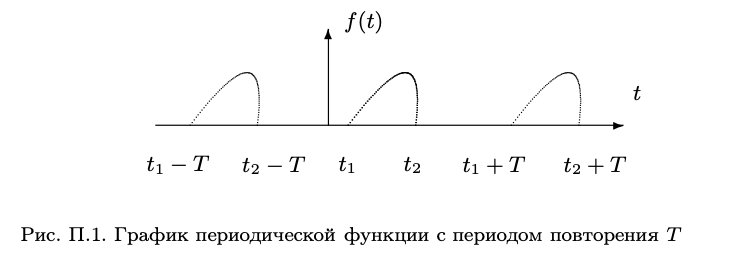
\includegraphics[width=0.7\linewidth]{./anat/1.jpg}\\
\end{center}

Пусть заданная функция $f(t)$ периодически повторяется с частотой $\Omega_{1}=2 \pi / T,$ где $T-$ период повторения $($ рис. $\Pi .1) .$ Её разложение в ряд Фурье имеет вид
$$
f(t)=\frac{a_{0}}{2}+\sum_{n=1}^{\infty}\left[a_{n} \cos \left(n \Omega_{1} t\right)+b_{n} \sin \left(n \Omega_{1} t\right)\right]
$$
или
$$
f(t)=\frac{A_{0}}{2}+\sum_{n=1}^{\infty} A_{n} \cos \left(n \Omega_{1} t-\psi_{n}\right)
$$
Здесь $a_{0} / 2=A_{0} / 2-$ постоянная составляюпдая (среднее значение) функции $f(t) ; a_{n}$ и $b_{n}-$ амплитуды косинусных и синусных членов разложе-ния. Они определяются выражениями
$$
\begin{array}{l}
a_{n}=\frac{2}{T} \int_{t_{1}}^{t_{1}+T} f(t) \cos \left(n \Omega_{1} t\right) d t \\
b_{n}=\frac{2}{T} \int_{t_{1}}^{t_{1}+T} f(t) \sin \left(n \Omega_{1} t\right) d t
\end{array}
$$

Точку начала интегрирования $t_{1}$ можно выбрать произвольно. В тех случаях, когда сигнал четен относительно $\mathrm{t}=0$, в тригонометрическои записи остаются только косинусные члены, т.к. все коэффициенты $b_{n}$ обращаются в нуль. Для нечетнои относительно $\mathrm{t}=0$ функции, наоборот, ряд состоит только из синусных членов.

Амплитуда $A_{n}$ и фаза $\psi_{n} n$ -й гармоники выражаются через $a_{n}$ и $b_{n}$ следуюшим образом:
$$
A_{n}=\sqrt{a_{n}^{2}+b_{n}^{2}} ; \quad \psi_{n}=\operatorname{arctg} \frac{b_{n}}{a_{n}}
$$
Как мы видим, спектр любой периодической функции состоит из набора гармонических колебаний с дискретными частотами: $\Omega_{1}, 2 \Omega_{1}, 3 \Omega_{1}$ $\ldots$ и постоянной составляющей, которую можно рассматривать как колебание с нулевой частотой $\left(0 \cdot \Omega_{1}\right) .$

Представим выражение в комплексной форме. Для этого заменим косинусы экспонентами в соответствии с формулой
$$
\cos \alpha=\frac{e^{i \alpha}+e^{-i \alpha}}{2}
$$
Подстановка даёт
$$
f(t)=\frac{1}{2}\left(A_{0}+\sum_{n=1}^{\infty} A_{n} e^{-i \psi_{n}} e^{i n \Omega_{1} t}+\sum_{n=1}^{\infty} A_{n} e^{i \psi_{n}} e^{-i n \Omega_{1} t}\right)
$$
Введём комплексные амплитуды $\tilde{A}_{n}$ и $\tilde{A}_{-n}$

$$
\tilde{A}_{n}=A_{n} e^{-i \psi_{n}} ; \quad \tilde{A}_{-n}=A_{n} e^{i \psi_{n}} ; \quad \tilde{A}_{0}=A_{0}
$$
Разложение $f(t)$ приобретает вид
$$
f(t)=\frac{1}{2} \sum_{n=-\infty}^{\infty} \tilde{A}_{n} e^{i n \Omega_{1} t}
$$

Как мы видим, введение отрицательных частот (типа $\mathrm{n} \Omega_{1}$ ) позволяет записать разложение Фурье особенно поостым образом.

Для расчёта комплексных амплитуд $A_{n}$ yмножим левую и правую части на $e^{-i k \Omega_{1} t}$ и проинтегрируем полученное равенство по времени на отрезке, равном одному периоду, например, от $t_{1}=0$ до $t_{2}=2 \pi / \Omega_{1} .$ В правой части обратятся в нуль все члены, кроме одного, соответствующего $n=k .$ Этот член даёт $A_{k} T / 2 .$ Имеем поэтому
$$
A_{k}=\frac{2}{T} \int_{0}^{T} f(t) e^{-i k \Omega_{1} t} d t
$$
Рассмотрим периодические функции, которые исследуются в нашей paбoтe.


\subsection{Периодическая последовательность прямоугольных импульсов}
C амплитудой $V_{0},$ длительностью $\tau,$ частотой повторения $f_{\text {повт }}=1 / T,$ где $T-$ период повторения импульсов.


Cреднее значение

$\langle V\rangle=\frac{a_{0}}{2}=\frac{A_{0}}{2}=\frac{1}{T} \int_{-\tau / 2}^{\tau / 2} V_{0} d t=V_{0} \frac{\tau}{T}$

Амплитуды косинусных составляющих равны

$$
a_{n}=\frac{2}{T} \int_{-\tau / 2}^{\tau / 2} V_{0} \cos \left(n \Omega_{1} t\right) d t=2 V_{0} \frac{\tau}{T} \frac{\sin \left(n \Omega_{1} \tau / 2\right)}{n \Omega_{1} \tau / 2} \sim \frac{\sin x}{x}
$$
Поскольку наша функция чётная, все амплитуды синусоидальных гармоник $b_{n}=0 .$ Спектр $F(\nu)$ последовательности прямоугольных импульсов представлен на рис. П.3. Амплитуды гармоник $A_{n}$ меняются по Закону $(\sin x) / x$
На рис. П.3 изображён спектр для случая, когда $T$ кратно $\tau .$ Назовём шириной спектра $\Delta \omega$ (или $\Delta \nu$ ) расстояние от главного максимума $(\nu=0)$ до первого нуля, возникающего, как нетрудно убедиться, при $\Omega_{1}=2 \pi / \tau$ При этом
$$
\Delta \omega \tau \simeq 2 \pi \quad \text { или } \quad \Delta \nu \Delta t \simeq 1
$$
Полученное соотношение взаимной связи интервалов $\Delta \nu$ и $\Delta t$ является
частным случаем соотношения неопределенности в квантовой механике. Несовместимость острой локализации волнового процесса во времени с узким спектром частот - явление широко известное в радиотехнике. Ширина селективной настройки $\Delta \nu$ радиоприёмника ограничивает приём радиосигналов Длительностью $t<1 / \Delta \nu$

 \begin{center}
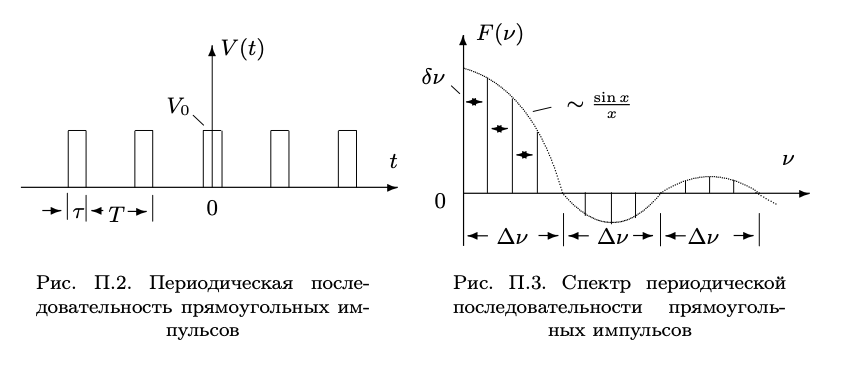
\includegraphics[width=0.7\linewidth]{./anat/2.jpg}\\
\end{center}

\subsection{Периодическая последовательность цугов}
Гармонического колебания $V_{0} \cos \left(\omega_{0} t\right)$ с длительностью цуга $\tau$ и периодом повторения $T$ (рис. $\Pi .4)$
 
Функция $f(t)$ снова является чётной относительно $t=0 .$ Амплитуда $n$ -й гармоники равна
$$
\begin{array}{c}
A_{n}=a_{n}=\frac{2}{T} \int_{-\tau / 2}^{\tau / 2} V_{0} \cos \left(\omega_{o} t\right) \cdot \cos \left(n \Omega_{1} t\right) d t= \\
=V_{0} \frac{\tau}{T}\left(\frac{\sin \left[\left(\omega_{0}-n \Omega_{1}\right) \frac{\tau}{2}\right]}{\left(\omega_{0}-n \Omega_{1}\right) \frac{\tau}{2}}+\frac{\sin \left[\left(\omega_{0}+n \Omega_{1}\right) \frac{\tau}{2}\right]}{\left(\omega_{0}+n \Omega_{1}\right) \frac{\tau}{2}}\right)
\end{array}
$$

Такое спектральное распределение F ($\omega$) для случая, когда $\frac T\tau$ равно целому числу, представлено на рис. П.5. Сравнивая спектр последовательности прямоугольных импульсов и спектр цугов (см. рис. П.3 и П.5), мы видим, что они аналогичны, но их максимумы сдвинуты по частоте на величину $\omega_0$.

\begin{center}
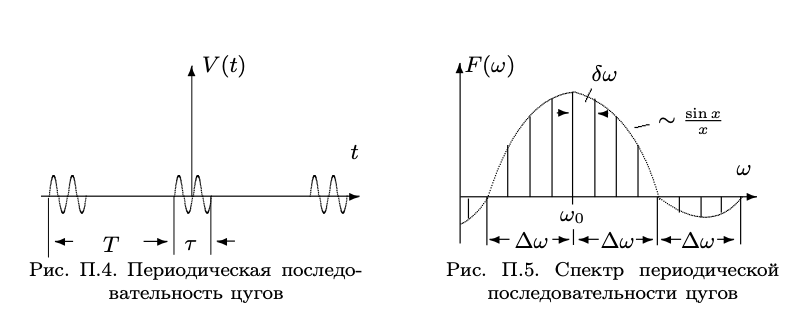
\includegraphics[width=0.7\linewidth]{./anat/3.jpg}\\
\end{center}

\subsection{Амплитудно-модулированные колебания.}

\begin{center}
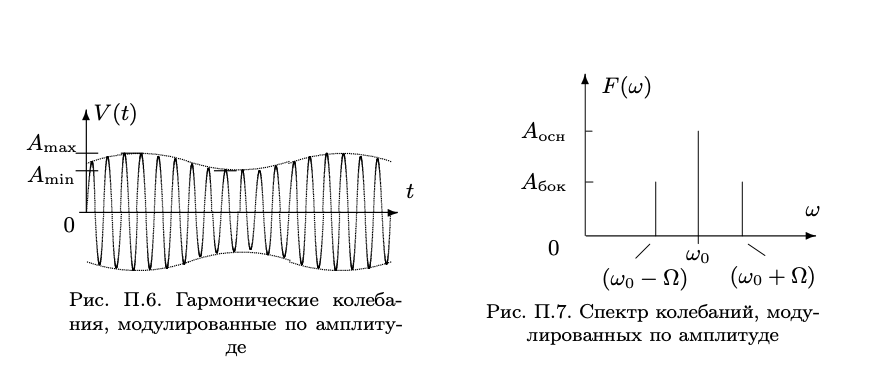
\includegraphics[width=0.7\linewidth]{./anat/4.jpg}\\
\end{center}
 Рассмотрим гармонические колебания высокой частоты $\omega_{0},$ амплитуда которых медленно меняется по гармоническому закону с частотой $\Omega\left(\Omega \ll \omega_{0}\right)$ (рис. П.6):
$$
f(t)=A_{0}[1+m \cos (\Omega t)] \cos (\omega t)
$$
Коэффициент $m$ называют глубиной модуляции. При $m<1$ амплитуда колебаний меняется от минимальной $A_{\min }=A_{0}(1-m)$ до максимальной $A_{\max }=A_{0}(1+m) .$ Глубина модулящии может быть представлена в виде
$$
m=\frac{A_{\max }-A_{\min }}{A_{\max }+A_{\min }}
$$
Простым тригонометрическим преобразованием можно найти спектр амплитудно-модулированных колебаний:
$$
\begin{aligned}
f(t) &=A_{0} \cos \left(\omega_{0} t\right)+A_{0} m \cos (\Omega t) \cos \left(\omega_{0} t\right)=\\
=A_{0} \cos \left(\omega_{0} t\right) &+\frac{A_{0} m}{2} \cos \left(\omega_{0}+\Omega\right) t+\frac{A_{0} m}{2} \cos \left(\omega_{0}-\Omega\right) t
\end{aligned}
$$

Спектр $F(\omega)$ таких колебаний содержит три составляюшцих (рис. П. 7$)$ Основная компонента представляет собой исходное немодулированное колебание с иесущей частотой $\omega_{0}$ и амплитудой $A_{\mathrm{ocн}}=A_{0}-$ первое слагаемое в правой части; боковые компоненты спектра соответствуют гармоническим колебаниям с частотами $\left(\omega_{0}+\Omega\right)$ и $\left(\omega_{0}-\Omega\right)-$ Второе и третье слагаемые. Амплитуды этих двух колебаний одинаковы и составляют $m / 2$ от амплитуды немодулированного колебания: $A_{\text {бок }}=A_{0} m / 2$


\section{Обработка данных}

\subsection{Периодические прямоугольные импульсы}

\begin{figure}[h!]
    \centering
    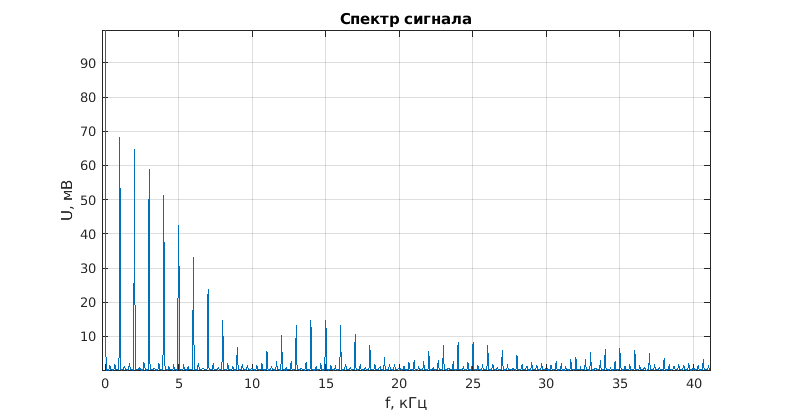
\includegraphics[width = 14 cm]{images/1_100_1.png}
    \caption{Спектр при $f_{\text{повт}} = 1$ кГц, $\tau = 100$ мкс}
\end{figure}

\begin{figure}[h!]
    \centering
    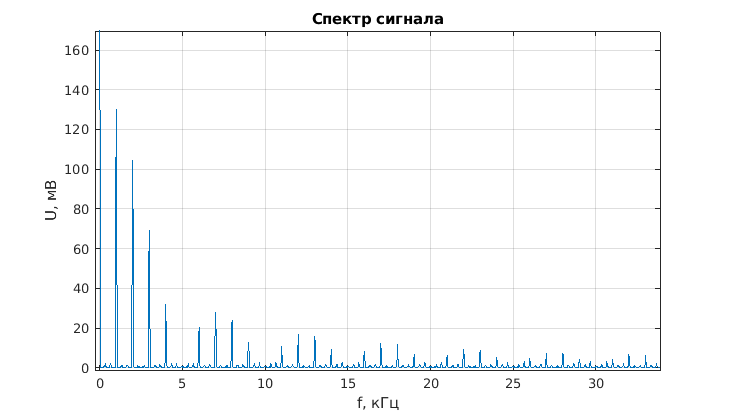
\includegraphics[width = 14 cm]{images/1_200_1.png}
    \caption{Спектр при $f_{\text{повт}} = 1$ кГц, $\tau = 200$ мкс}
\end{figure}

\begin{figure}[h!]
    \centering
    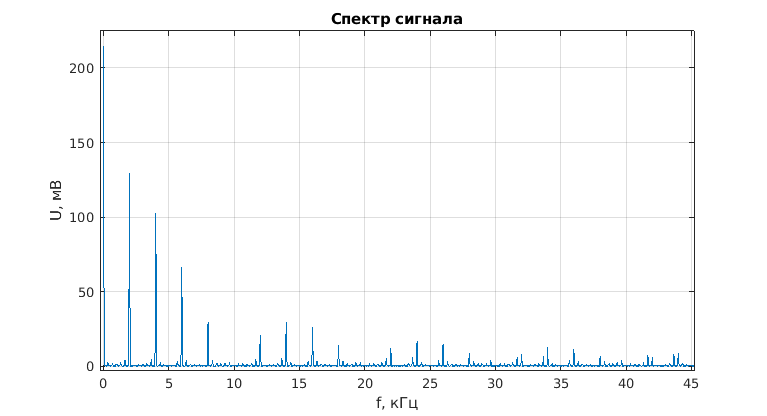
\includegraphics[width = 14 cm]{images/1_100_2.png}
    \caption{Спектр при $f_{\text{повт}} = 2$ кГц, $\tau = 100$ мкс}
\end{figure}

\begin{figure}[h!]
    \centering
    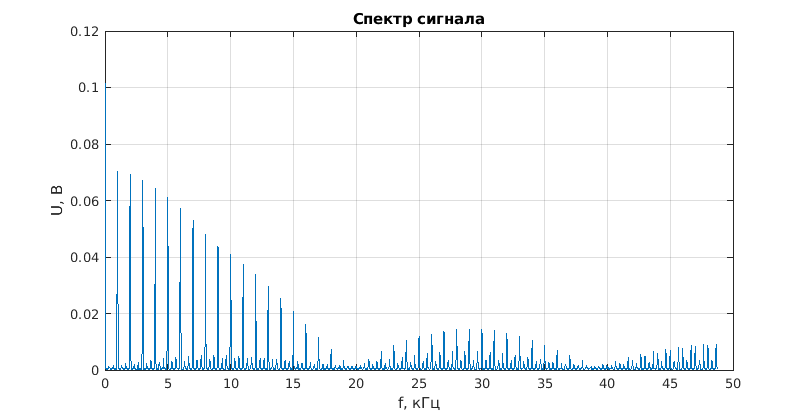
\includegraphics[width = 14 cm]{images/1_50_1.png}
    \caption{Спектр при $f_{\text{повт}} = 1$ кГц, $\tau = 50$ мкс}
\end{figure}

При фиксированной частоте $f_{\text{повт}} = 1$ кГц будем менять $\tau$, при этом будет меняться ширина спектра. Зафиксируем наблюдения в таблице.

\begin{table}[]
    \centering
    \begin{tabular}{|c|l|l|l|l|l|l|l|l|l|}
        \hline
        \textbf{$\tau$, мкс}           & 40 & 60    & 80   & 100 & 120  & 140  & 160  & 180  & 200 \\ \hline
        \textbf{$\Delta \nu$, кГц}     & 25 & 16,5  & 12,5 & 10  & 8,5  & 7    & 6,5  & 5,5  & 5   \\ \hline
        \textbf{$\frac{1}{\tau}$, кГц} & 25 & 16,66 & 12,5 & 10  & 8,33 & 7,14 & 6,25 & 5,56 & 5   \\ \hline
    \end{tabular}
    \caption{Зависимость ширины спектра от времени длительности импульса}
\end{table}

Построим график зависимости $\Delta \nu (\frac{1}{\tau})$:

\begin{figure}[h!]
    \centering
    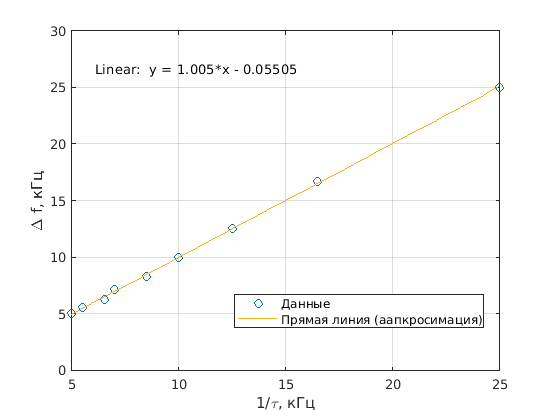
\includegraphics[width = 13 cm]{images/1_appr.png}
    \caption{Зависимость $\Delta \nu (\frac{1}{\tau})$}
\end{figure}

Из графика следует выоплнение соотношения неопределённости для прямяугольных импульсов: $\Delta \nu \cdot \tau = \approx 1$.

\subsection{Периодическая последовательность цугов}

Установим несущую частоту цугов $\nu_0 = 25$ кГц, частота запуска цугов $f_{\text{повт}} = 1$ кГц с длительностью импульса $\tau = 100$ мкс.

Проанализируем, как меняется спектр при изменении длительности импульса цуга.

\begin{figure}[h!]
    \centering
    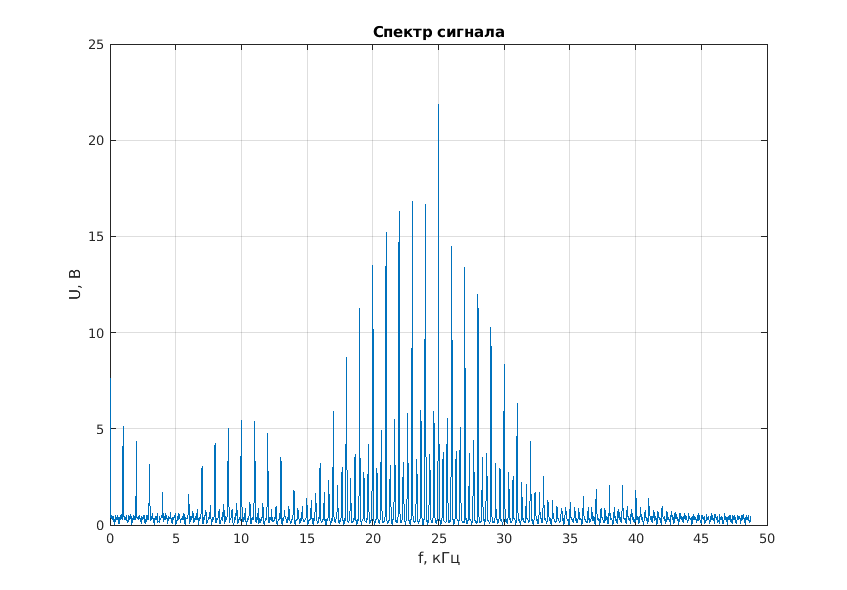
\includegraphics[width = 14 cm]{images/2_100_1.png}
    \caption{Спектр при $\nu_0 = 25$ кГц, $\tau = 100$ мкс}
\end{figure}

\begin{figure}[h!]
    \centering
    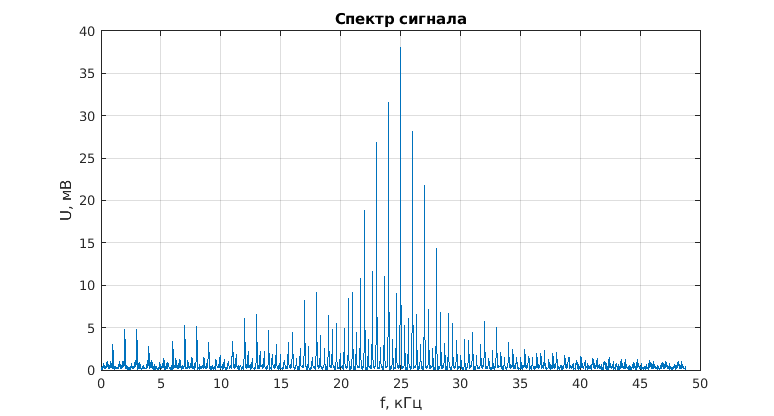
\includegraphics[width = 14 cm]{images/2_200_1.png}
    \caption{Спектр при $\nu_0 = 25$ кГц, $\tau = 200$ мкс}
\end{figure}

Теперь проанализируем, как меняется спектр при изменении несущей частоты.

\begin{figure}[h!]
    \centering
    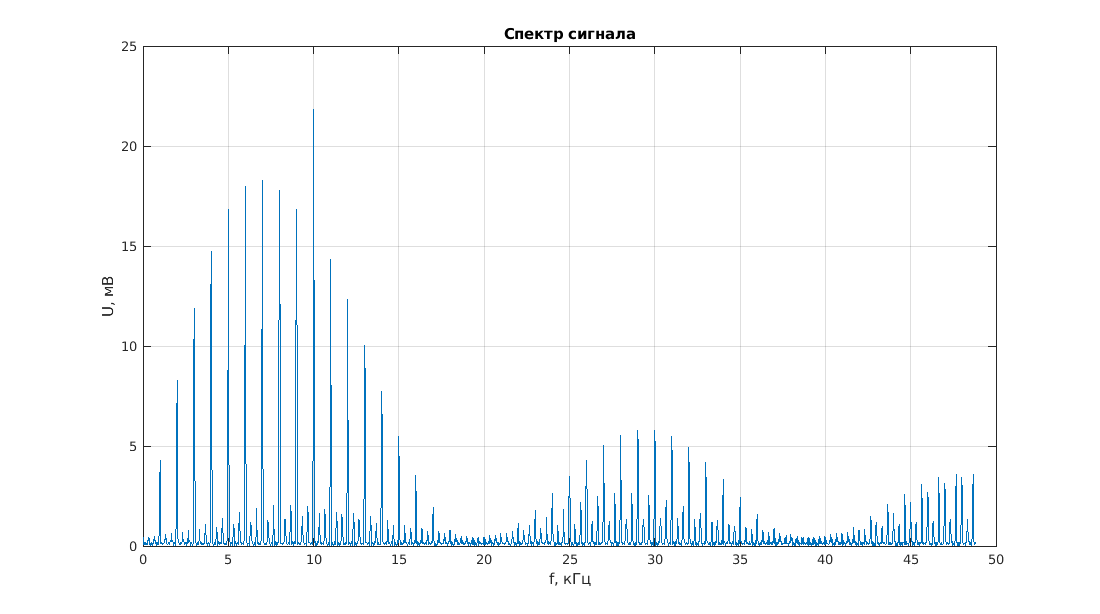
\includegraphics[width = 14 cm]{images/2_10k.png}
    \caption{Спектр при $\nu_0 = 10$ кГц, $\tau = 100$ мкс}
\end{figure}

\begin{figure}[h!]
    \centering
    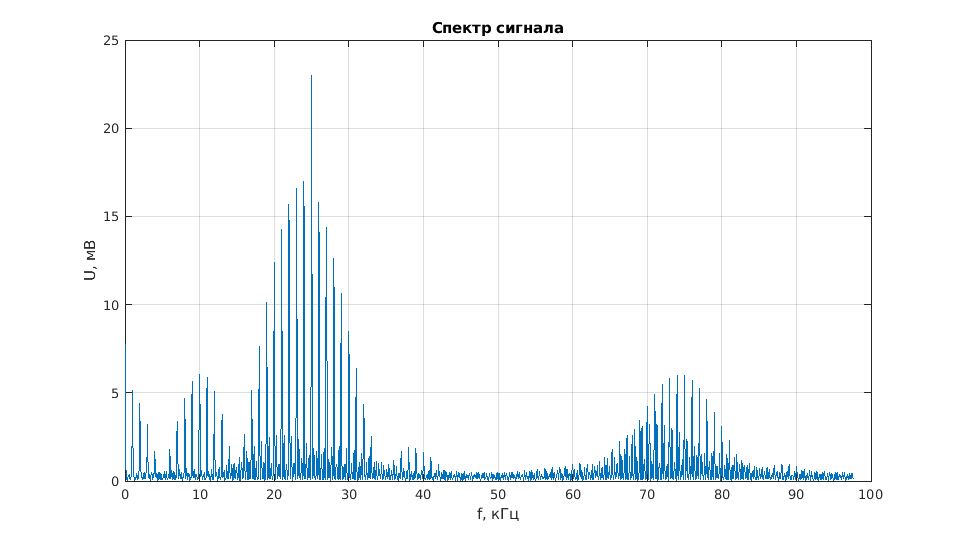
\includegraphics[width = 14 cm]{images/2_25k.png}
    \caption{Спектр при $\nu_0 = 25$ кГц, $\tau = 100$ мкс}
\end{figure}

\begin{figure}[h!]
    \centering
    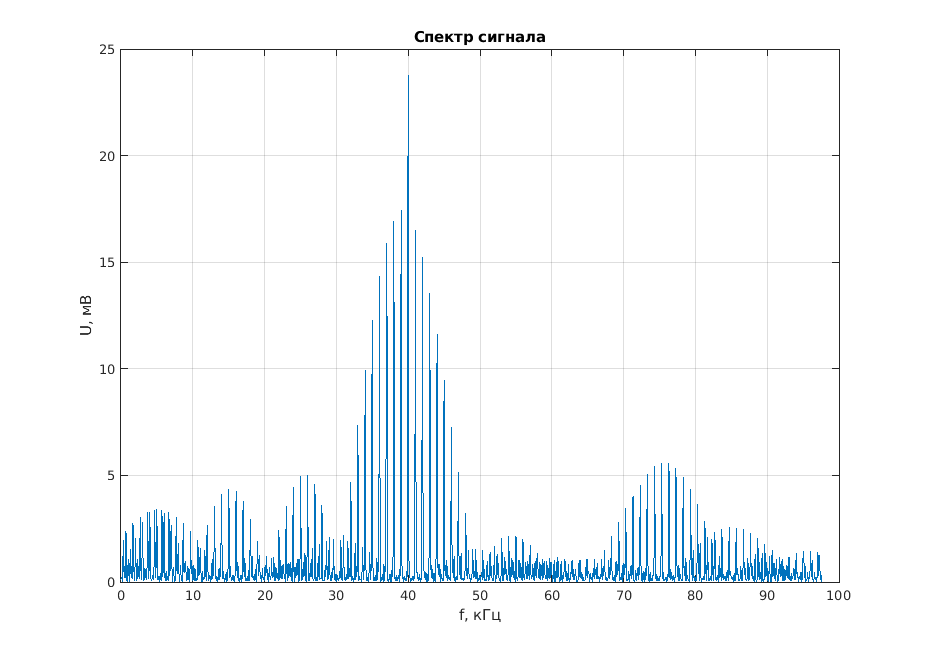
\includegraphics[width = 14 cm]{images/2_40k.png}
    \caption{Спектр при $\nu_0 = 40$ кГц, $\tau = 100$ мкс}
\end{figure}

Установим несущую частоту $\nu_0 = 30$ кГц при $\tau = 100$ Гц, варируя частоту запуска цугов. Снимем зависиимость расстояния между соседними спектральными компонентами от частоты повтоения цугов:

\begin{table}[]
    \centering
    \begin{tabular}{|c|l|l|l|l|l|l|l|l|l|}
        \hline
        \textbf{$\delta \nu$, кГц}      & 0,5 & 1  & 2 & 4  & 5  \\ \hline
        \textbf{$f_{\text{повт}}$, кГц} & 0,5 & 1  & 2 & 4  & 5  \\ \hline
    \end{tabular}
    \caption{Зависимость расстояния между компонентами спектра от частоты повторения цугов}
\end{table}

Данные по расстоянию между компонентами спектра получены по более, чем 80 точек данных, и с точностью до погрешности генератора совпадают со значениями частоты повторения цугов $f_{\text{повт}}$.

Получается, что $\delta \nu = k f_{\text{повт}}$, где $k \approx 1$. Из теории следует, что значения двух величин совпадают, значит экспериментальная зависимость верна.

И для прямугольных импульсов, и для цугов при повышении частоты повторения импульсов увеличивается расстояние между компонентами спектра, а при повышении длительности импульса уменьшается ширина спектра. Разница между графиками спектров прямугольного импульса и цуга в том, что спектр цугаа смещён на значение несущей частоты в сторону поовышения частоты. То есть при устрмлении несущей частоты к нулю графики наложатся друг на друга.

\subsection{Амплитудно-модулированные колебания}

Установим синусоидальный сигнал частоты $\nu_0 = 25$ кГц, амплитуды $0,5$ В. Подключим модуляцию к этому сигналу амплитуды $0,1$ В и частоты $\nu = 1$ кГц.

Меняя глубину модуляции до 1, измерим следующие значения:

\begin{table}[h!]
    \centering
    \begin{tabular}{|c|c|c|c|c|c|c|c|}
        \hline
        \textbf{$A_{min}$, мВ}                           & 450   & 375   & 300   & 225   & 150   & 75    & 0     \\ \hline
        \textbf{$A_{max}$, мВ}                           & 550   & 625   & 700   & 775   & 850   & 925   & 1000  \\ \hline
        \textbf{$m$}                                     & 0,1   & 0,25  & 0,4   & 0,55  & 0,7   & 0,85  & 1     \\ \hline
        \textbf{$A_{\text{бок}}$, мВ}                    & 17    & 43    & 68    & 94    & 120   & 147   & 174   \\ \hline
        \textbf{$A_{\text{осн}}$, мВ}                    & 343   & 341   & 342   & 342   & 340   & 342   & 341   \\ \hline
        \textbf{$\frac{A_{\text{бок}}}{A_{\text{осн}}}$} & 0,496 & 0,126 & 0,199 & 0,275 & 0,353 & 0,430 & 0,510 \\ \hline
    \end{tabular}
    \caption{Зависимость $\frac{A_{\text{бок}}}{A_{\text{осн}}}$ от $m$}
\end{table}

Построим график зависимости.

\begin{figure}[!h]
    \centering
    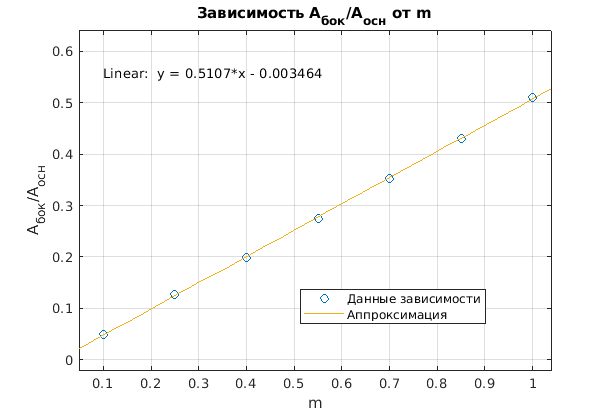
\includegraphics[width = 13 cm]{images/3_appr.png}
    \caption{График зависимости $\frac{A_{\text{бок}}}{A_{\text{осн}}}$ от $m$}
\end{figure}

Получилось значение $k = 0,511 \pm 0,021$, согласно же теории это значение должно равняться $0,5$. То есть получилось верное соотношение амплитуд при различных модуляциях.

При увеличении частоты модуляции две боковые гармоники отдаляются от основной по величине на спектре.

\subsection{Частотная модуляция}

Установим синусоидальный сигнал с частотой $\nu = 25$ кГц с синусоидальной модуляцией частоты $1$ кГц с девиацией частоты $100$ Гц.

Меняя девиацию, снимем зависимость амплитуд гармоник от её значения.

\begin{table}[!h]
    \centering
    \begin{tabular}{|c|c|c|c|c|c|c|c|l|l|l|}
        \hline
        \textbf{$\Delta f_m$, кГц}       & 0,1   & 0,2   & 0,3   & 0,4   & 0,5   & 0,6   & 0,7   & 0,8   & 0,9   & 1     \\ \hline
        \textbf{$A_0$, мВ}               & 338   & 335   & 331   & 325   & 318   & 309   & 299   & 287   & 273   & 260   \\ \hline
        \textbf{$A_{+-1}$, мВ}           & 17    & 33    & 50    & 67    & 83    & 97    & 112   & 125   & 138   & 150   \\ \hline
        \textbf{$A_{+-2}$, мВ}           & 0     & 2     & 4     & 7     & 10    & 15    & 20    & 26    & 32    & 38    \\ \hline
        \textbf{$\beta$}                 & 0,1   & 0,2   & 0,3   & 0,4   & 0,5   & 0,6   & 0,7   & 0,8   & 0,9   & 1     \\ \hline
        \textbf{$\frac{A_{+-1}}{A_{0}}$} & 0,050 & 0,099 & 0,151 & 0,206 & 0,261 & 0,314 & 0,375 & 0,436 & 0,505 & 0,577 \\ \hline
    \end{tabular}
\end{table}

Построим график зависимости $\frac{A_{+-1}}{A_{0}}$ от $\beta$:

\begin{figure}[!h]
    \centering
    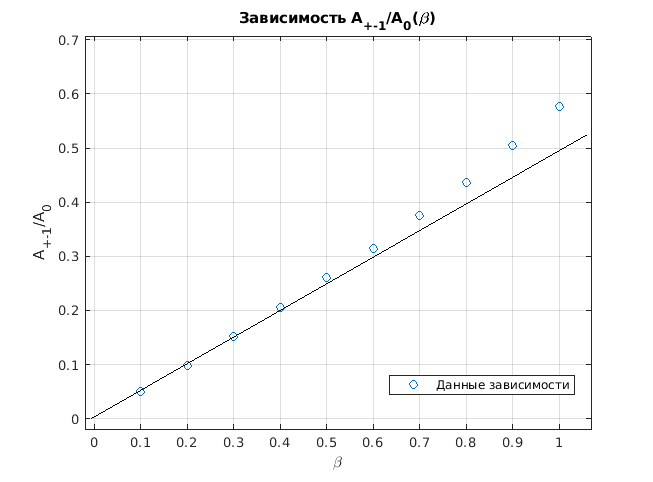
\includegraphics[width = 13 cm]{images/4_appr.png}
    \caption{График зависимости $\frac{A_{+-1}}{A_{0}}$ от $\beta$}
\end{figure}

Предельная кривая, построенная при $\beta \ll 1$, даёт отношение боковых гармоник к основной $k = 0,5$, что и соответсвуте теоретической формуле, выведенной в приближении $\beta \ll 1$. При этом значения $\beta \geqslant 0,9$ дают отклонение от построенной прямой больше, чем $10$ \%.

При дальнейшей увеличении частоты девиации получим более сложные спектры:

\newpage

\begin{figure}[!h]
    \centering
    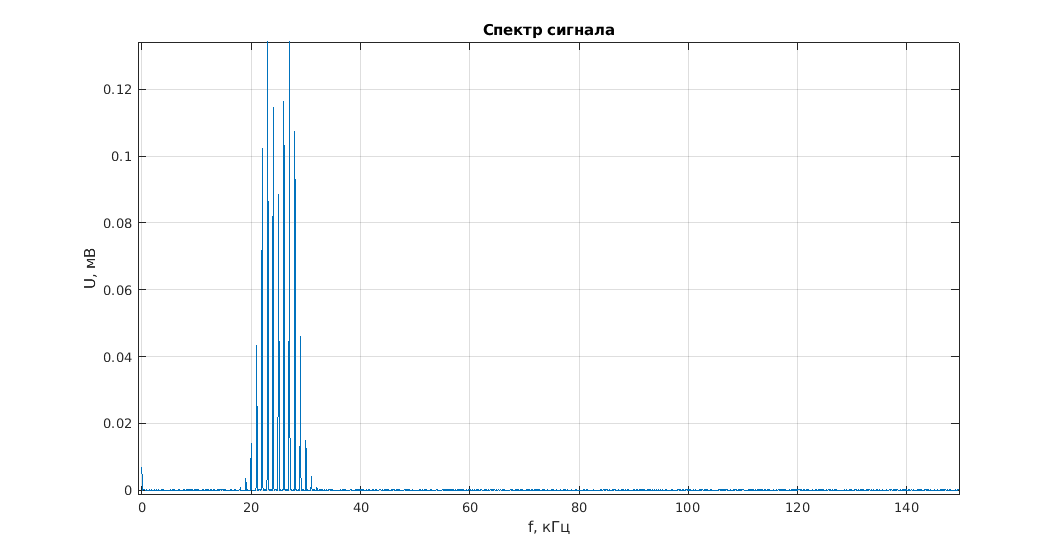
\includegraphics[width = 15 cm]{images/4_3.png}
    \caption{Спектр при частоте девиации $\Delta f_m = 3$ кГц}
\end{figure}


\begin{figure}[!h]
    \centering
    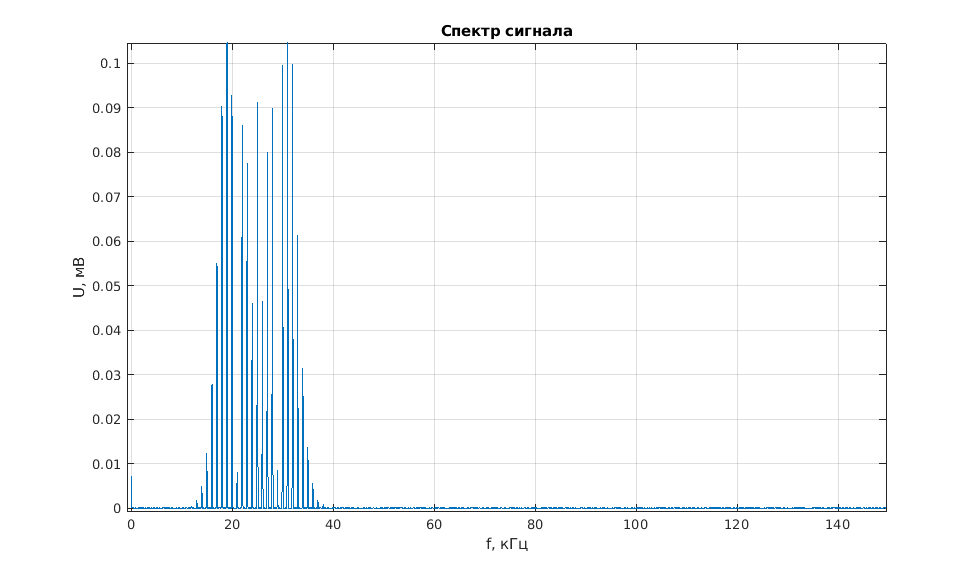
\includegraphics[width = 15 cm]{images/4_7.5.png}
    \caption{Спектр при частоте девиации $\Delta f_m = 7,5$ кГц}
\end{figure}

\newpage

\section{Заключение}

В ходе выполнения работы теоретическое описание спектров исследуемых сигналов подтвердилось на основе их изучения с помощью генератора и осциллографа.
 
\section{Литература}

\begin{enumerate}

\item \textbf{Лабораторный практикум по общей физике:} учеб. пособие. В трёх томах. Т. 2. Электричество и магнетизм /
Никулин М. Г., Попов П. В., Нозик А. А., и др.; под ред. А. В. Мак­симычева, М. Г. Никулина. — 2-е изд., перераб. и доп. — Москва : МФТИ, 2019. — 370 с.
ISBN 978-5-7417-0709-8 (Т. 2. Электричество и магнетизм)
\end{enumerate}		
		

\end{document}
